% Options for packages loaded elsewhere
% Options for packages loaded elsewhere
\PassOptionsToPackage{unicode}{hyperref}
\PassOptionsToPackage{hyphens}{url}
\PassOptionsToPackage{dvipsnames,svgnames,x11names}{xcolor}
%
\documentclass[
  letterpaper,
  DIV=11,
  numbers=noendperiod]{scrreprt}
\usepackage{xcolor}
\usepackage{amsmath,amssymb}
\setcounter{secnumdepth}{5}
\usepackage{iftex}
\ifPDFTeX
  \usepackage[T1]{fontenc}
  \usepackage[utf8]{inputenc}
  \usepackage{textcomp} % provide euro and other symbols
\else % if luatex or xetex
  \usepackage{unicode-math} % this also loads fontspec
  \defaultfontfeatures{Scale=MatchLowercase}
  \defaultfontfeatures[\rmfamily]{Ligatures=TeX,Scale=1}
\fi
\usepackage{lmodern}
\ifPDFTeX\else
  % xetex/luatex font selection
\fi
% Use upquote if available, for straight quotes in verbatim environments
\IfFileExists{upquote.sty}{\usepackage{upquote}}{}
\IfFileExists{microtype.sty}{% use microtype if available
  \usepackage[]{microtype}
  \UseMicrotypeSet[protrusion]{basicmath} % disable protrusion for tt fonts
}{}
\makeatletter
\@ifundefined{KOMAClassName}{% if non-KOMA class
  \IfFileExists{parskip.sty}{%
    \usepackage{parskip}
  }{% else
    \setlength{\parindent}{0pt}
    \setlength{\parskip}{6pt plus 2pt minus 1pt}}
}{% if KOMA class
  \KOMAoptions{parskip=half}}
\makeatother
% Make \paragraph and \subparagraph free-standing
\makeatletter
\ifx\paragraph\undefined\else
  \let\oldparagraph\paragraph
  \renewcommand{\paragraph}{
    \@ifstar
      \xxxParagraphStar
      \xxxParagraphNoStar
  }
  \newcommand{\xxxParagraphStar}[1]{\oldparagraph*{#1}\mbox{}}
  \newcommand{\xxxParagraphNoStar}[1]{\oldparagraph{#1}\mbox{}}
\fi
\ifx\subparagraph\undefined\else
  \let\oldsubparagraph\subparagraph
  \renewcommand{\subparagraph}{
    \@ifstar
      \xxxSubParagraphStar
      \xxxSubParagraphNoStar
  }
  \newcommand{\xxxSubParagraphStar}[1]{\oldsubparagraph*{#1}\mbox{}}
  \newcommand{\xxxSubParagraphNoStar}[1]{\oldsubparagraph{#1}\mbox{}}
\fi
\makeatother


\usepackage{longtable,booktabs,array}
\usepackage{calc} % for calculating minipage widths
% Correct order of tables after \paragraph or \subparagraph
\usepackage{etoolbox}
\makeatletter
\patchcmd\longtable{\par}{\if@noskipsec\mbox{}\fi\par}{}{}
\makeatother
% Allow footnotes in longtable head/foot
\IfFileExists{footnotehyper.sty}{\usepackage{footnotehyper}}{\usepackage{footnote}}
\makesavenoteenv{longtable}
\usepackage{graphicx}
\makeatletter
\newsavebox\pandoc@box
\newcommand*\pandocbounded[1]{% scales image to fit in text height/width
  \sbox\pandoc@box{#1}%
  \Gscale@div\@tempa{\textheight}{\dimexpr\ht\pandoc@box+\dp\pandoc@box\relax}%
  \Gscale@div\@tempb{\linewidth}{\wd\pandoc@box}%
  \ifdim\@tempb\p@<\@tempa\p@\let\@tempa\@tempb\fi% select the smaller of both
  \ifdim\@tempa\p@<\p@\scalebox{\@tempa}{\usebox\pandoc@box}%
  \else\usebox{\pandoc@box}%
  \fi%
}
% Set default figure placement to htbp
\def\fps@figure{htbp}
\makeatother





\setlength{\emergencystretch}{3em} % prevent overfull lines

\providecommand{\tightlist}{%
  \setlength{\itemsep}{0pt}\setlength{\parskip}{0pt}}



 


\KOMAoption{captions}{tableheading}
\makeatletter
\@ifpackageloaded{bookmark}{}{\usepackage{bookmark}}
\makeatother
\makeatletter
\@ifpackageloaded{caption}{}{\usepackage{caption}}
\AtBeginDocument{%
\ifdefined\contentsname
  \renewcommand*\contentsname{Table of contents}
\else
  \newcommand\contentsname{Table of contents}
\fi
\ifdefined\listfigurename
  \renewcommand*\listfigurename{List of Figures}
\else
  \newcommand\listfigurename{List of Figures}
\fi
\ifdefined\listtablename
  \renewcommand*\listtablename{List of Tables}
\else
  \newcommand\listtablename{List of Tables}
\fi
\ifdefined\figurename
  \renewcommand*\figurename{Figure}
\else
  \newcommand\figurename{Figure}
\fi
\ifdefined\tablename
  \renewcommand*\tablename{Table}
\else
  \newcommand\tablename{Table}
\fi
}
\@ifpackageloaded{float}{}{\usepackage{float}}
\floatstyle{ruled}
\@ifundefined{c@chapter}{\newfloat{codelisting}{h}{lop}}{\newfloat{codelisting}{h}{lop}[chapter]}
\floatname{codelisting}{Listing}
\newcommand*\listoflistings{\listof{codelisting}{List of Listings}}
\makeatother
\makeatletter
\makeatother
\makeatletter
\@ifpackageloaded{caption}{}{\usepackage{caption}}
\@ifpackageloaded{subcaption}{}{\usepackage{subcaption}}
\makeatother
\usepackage{bookmark}
\IfFileExists{xurl.sty}{\usepackage{xurl}}{} % add URL line breaks if available
\urlstyle{same}
\hypersetup{
  pdftitle={Muhammad Azikra Wira Pratama},
  pdfauthor={18224089 Muhammad Azikra Wira Pratama},
  colorlinks=true,
  linkcolor={blue},
  filecolor={Maroon},
  citecolor={Blue},
  urlcolor={Blue},
  pdfcreator={LaTeX via pandoc}}


\title{Muhammad Azikra Wira Pratama}
\usepackage{etoolbox}
\makeatletter
\providecommand{\subtitle}[1]{% add subtitle to \maketitle
  \apptocmd{\@title}{\par {\large #1 \par}}{}{}
}
\makeatother
\subtitle{Tugas Portofolio Komunikasi Interpersonal dan Publik}
\author{18224089 Muhammad Azikra Wira Pratama}
\date{2025-10-05}
\begin{document}
\maketitle

\renewcommand*\contentsname{Table of contents}
{
\hypersetup{linkcolor=}
\setcounter{tocdepth}{2}
\tableofcontents
}

\bookmarksetup{startatroot}

\chapter*{Hallo Semua}\label{hallo-semua}
\addcontentsline{toc}{chapter}{Hallo Semua}

\markboth{Hallo Semua}{Hallo Semua}

\begin{figure}[H]

{\centering \pandocbounded{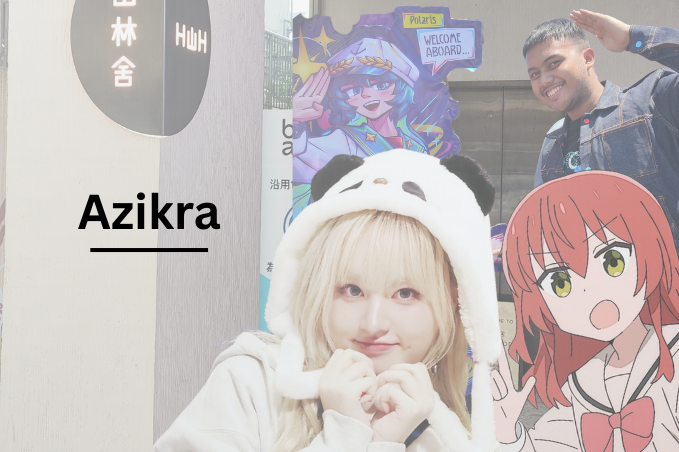
\includegraphics[keepaspectratio]{images/CoverIstri.png}}

}

\caption{Profil diri}

\end{figure}%

Muhammad Azikra Wira Pratama, yang akrab dipanggil ``Zik'' atau
``Zikra'', merupakan mahasiswa Sekolah Teknik Elektro dan Informatika --
Komputasi, Institut Teknologi Bandung (Angkatan 2024), dengan program
studi Sistem dan Teknologi Informasi (kode II).

Zikra lahir di Pekanbaru pada tahun 2006 dan saat ini berdomisili di
Cimahi.

\begin{center}\rule{0.5\linewidth}{0.5pt}\end{center}

\section*{Connect with Me}\label{connect-with-me}
\addcontentsline{toc}{section}{Connect with Me}

\markright{Connect with Me}

\begin{itemize}
\tightlist
\item
  Email :
  \href{mailto:18224089@std.stei.itb.ac.id}{\nolinkurl{18224089@std.stei.itb.ac.id}}
\end{itemize}

\bookmarksetup{startatroot}

\chapter{UTS-1 All About Me}\label{uts-1-all-about-me}

\begin{center}\rule{0.5\linewidth}{0.5pt}\end{center}

\section{Identitas Diri}\label{identitas-diri}

\begin{longtable}[]{@{}ll@{}}
\toprule\noalign{}
\textbf{Nama} & Muhammad Azikra Wira Pratama \\
\midrule\noalign{}
\endhead
\bottomrule\noalign{}
\endlastfoot
\textbf{Program Studi} & Sistem dan Teknologi Informasi \\
\textbf{NIM} & 18224089 \\
\textbf{Tujuan} & Memperkenalkan sosok diri secara reflektif \\
\end{longtable}

\begin{center}\rule{0.5\linewidth}{0.5pt}\end{center}

\section{Refleksi Diri}\label{refleksi-diri}

Portofolio ini saya buat sebagai sarana untuk \textbf{merefleksikan diri
saya sebenarnya} bagaimana saya \textbf{memandang diri sendiri}, dan
bagaimana saya \textbf{menampilkan diri kepada orang lain}.\\
Melalui proses ini, saya berusaha untuk memahami siapa saya di balik
peran dan ekspektasi sosial yang saya jalani setiap hari.

Saya percaya bahwa dengan memahami diri secara jujur, saya dapat
\textbf{hidup dengan lebih autentik, selaras dengan nilai-nilai yang
saya yakini}, dan berinteraksi dengan orang lain secara lebih terbuka
dan bermakna.

\begin{center}\rule{0.5\linewidth}{0.5pt}\end{center}

\begin{quote}
\emph{``Hujan tidak selalu berarti sedih, kadang hanya cara dunia
mengingatkan kita untuk berhenti sejenak.''}
\end{quote}

\begin{center}\rule{0.5\linewidth}{0.5pt}\end{center}

\section{Siapa saya}\label{siapa-saya}

\begin{figure}[H]

{\centering 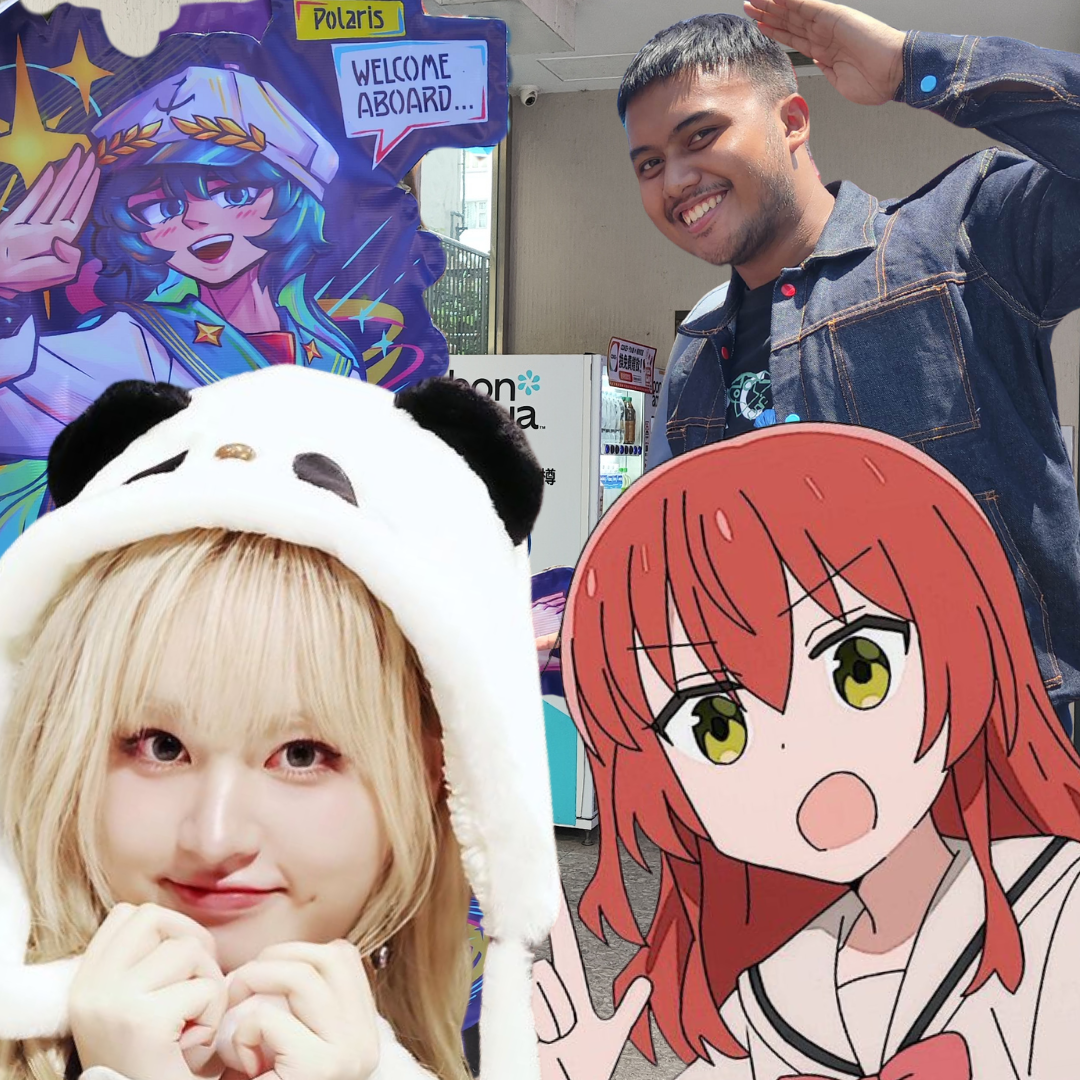
\includegraphics[width=0.6\linewidth,height=\textheight,keepaspectratio]{All_about_me/../images/Identitas.png}

}

\caption{Profil diri}

\end{figure}%

Kenalin saya \textbf{Muhammad Azikra Wira Pratama}, atau biasa dipanggil
\textbf{Zik/Zikra}. Saya mahasiswa dari program studi Sistem dan
Teknologi Informasi (II), Fakultas STEI, angkatan 2024.

Saya lahir di \textbf{Pekanbaru} dan kini tinggal di \textbf{Cimahi}.
Walau saya berdomisili Cimahi, saya sangat sering pergi ke
\textbf{Bandung}.

\begin{center}\rule{0.5\linewidth}{0.5pt}\end{center}

\section{Apa yang Membentuk Saya}\label{apa-yang-membentuk-saya}

Sejak kecil, saya selalu tertarik dengan bidang teknologi yang dimulai
dari kesukaan saya ketika memainkan gim. Bidang ini saya telusuri
sedikit-sedikit hingga jadi tertarik untuk masuk ke jurusan di dunia
informatika. Kampus yang saya impikan itu \textbf{ITB} dan ketika
mengetahui bahwa terdapat fakultas \textbf{STEI} saya menjadikan hal
tersebut target selama menempuh pendidikan \textbf{SMA}.

\begin{center}\rule{0.5\linewidth}{0.5pt}\end{center}

\section{Bagaimana Saya Melihat Diri}\label{bagaimana-saya-melihat-diri}

Saya orang yang \textbf{pendiam di awal}, tapi \textbf{kalau sudah
nyaman akan sangat ekpresif}. Saya cenderung memilih diam jika ada
diberikan waktu untuk berpikir dalam memutuskan suatu hal.

Hal kecil yang terjadi kadang saya perhatikan seperti apa respons
spontan yang diberikan ketika saya berbicara, bertindak, atau bercanda.
Saya berusaha untuk memerhatikan diri agar tidak menyinggung perasaan
orang. Hal tersebutlah yang membuat saya belajar mengenai
\textbf{Komunikasi diri}, tentang bagaimana jujur tanpa harus membuka
hal pribadi.

\begin{center}\rule{0.5\linewidth}{0.5pt}\end{center}

\section{Sisi Ringan Saya}\label{sisi-ringan-saya}

Mengenai hal tadi selain memerhatikan hal kecil dari diri saya, kadang
saya memerhatikan juga aktivitas unik dari orang di sekitar saya
terutama teman-teman saya.

Hal ini sering saya jadikan seperti upaya saya untuk menjadi lebih dekat
dan terhubung dengan mereka. Saya bisa menggunakan teknik tersebut
dengan pembicaraan ringan, bercanda, dan hal menarik lainnya.

Selain kebiasaan tersebut dalam lingkup sosial, ketika sedang bersantai
sendiri saya sering mendengarkan lagu tenang atau sedih. Saya cenderung
menyelam dalam perasaan sendiri untuk refleksi atau sekedar istirahat
dari lingkup sosial.

\begin{center}\rule{0.5\linewidth}{0.5pt}\end{center}

\section{Refleksi dan Nilai Hidup}\label{refleksi-dan-nilai-hidup}

Bagi saya, \textbf{komunikasi diri} adalah tentang keberanian untuk
jujur pada diri sendiri. Saya belajar bahwa \textbf{menerima kelemahan
bukan tanda menyerah}, tapi langkah pertama untuk tumbuh.

Saya ingin hidup dengan prinsip:

\begin{quote}
\emph{``Tidak harus selalu benar, tapi harus selalu mau belajar.''}
\end{quote}

Dengan memahami diri, saya berharap bisa \textbf{lebih autentik,
konsisten dengan nilai yang saya yakini}, dan membawa empati ke setiap
hubungan dalam kehidupan.

\begin{center}\rule{0.5\linewidth}{0.5pt}\end{center}

\section{Penutup}\label{penutup}

Portofolio ini bukan hanya tentang siapa saya sekarang, tapi juga
tentang siapa saya ingin jadi.\\
Mungkin hujan akan tetap turun, tapi selama saya melangkah dengan jujur,
saya tahu matahari akan muncul pada waktunya.

\bookmarksetup{startatroot}

\chapter{UTS-2 My Songs for You}\label{uts-2-my-songs-for-you}

\section{This is The Song}\label{this-is-the-song}

\url{https://www.youtube.com/embed/LHCob76kigA}

\begin{quote}
\textbf{Lukas Graham -- ``7 Years''}\\
\emph{A reflection on growing up, dreams, and family.}
\end{quote}

\section{Lirik Lagu}\label{lirik-lagu}

{[}Chorus{]} Once, I was seven years old, my mama told me ``Go make
yourself some friends or you'll be lonely'' Once, I was seven years old

{[}Verse 1{]} It was a big, big world, but we thought we were bigger
Pushing each other to the limits, we were learnin' quicker By eleven,
smokin' herb and drinkin' burnin' liquor Never rich, so we were out to
make that steady figure

{[}Chorus{]} Once, I was eleven years old, my daddy told me ``Go get
yourself a wife or you'll be lonely'' Once, I was eleven years old

{[}Verse 2{]} I always had that dream like my daddy before me So I
started writin' songs, I started writin' stories Something about that
glory just always seemed to bore me 'Cause only those I really love will
ever really know me

{[}Chorus{]} Once, I was twenty years old, my story got told Before the
mornin' sun, when life was lonely Once, I was twenty years old (Lukas
Graham!)

{[}Verse 3{]} I only see my goals, I don't believe in failure 'Cause I
know the smallest voices, they can make it major I got my boys with me,
at least those in favor And if we don't meet before I leave, I hope I'll
see you later

{[}Chorus{]} Once, I was twenty years old, my story got told I was
writin' 'bout everything I saw before me Once, I was twenty years old

{[}Bridge{]} Soon, we'll be thirty years old, our songs have been sold
We've traveled around the world and we're still roamin' Soon, we'll be
thirty years old

{[}Verse 4{]} I'm still learnin' about life, my woman brought children
for me So I can sing them all my songs and I can tell them stories Most
of my boys are with me, some are still out seekin' glory And some I had
to leave behind, my brother, I'm still sorry

{[}Chorus{]} Soon, I'll be sixty years old, my daddy got sixty-one
Remember life and then your life becomes a better one I made a man so
happy when I wrote a letter once I hope my children come and visit once
or twice a month

{[}Breakdown{]} Soon, I'll be sixty years old, will I think the world is
cold Or will I have a lot of children who can warm me? Soon, I'll be
sixty years old Soon, I'll be sixty years old, will I think the world is
cold Or will I have a lot of children who can warm me? Soon, I'll be
sixty years old

{[}Chorus{]} Once, I was seven years old, my mama told me ``Go make
yourself some friends or you'll be lonely'' Once, I was seven years old
Once, I was seven years old

\begin{center}\rule{0.5\linewidth}{0.5pt}\end{center}

\section{Kenapa lagu ini?}\label{kenapa-lagu-ini}

Saya memilih lagu ini karena ini cocok untuk direnungkan pada setiap
pilihan hidup saya dan perkembangan saya.\\
Bagi saya, tema terkuatnya adalah makna bertambah usia.

Awalnya lagu ini adalah pengisi hiburan dikala bosan saat di kelas. Guru
SD saat itu bernama Pak Yanyan sering memutarkan lagu ini untuk menambah
suasana ramai dan berwarna dalam kelas yang saat itu sedang santai.
Seiring waktu berjalan setelah lulus dari jenjang SD, saya semakin
jarang memutar lagu ini. Terkadang mengingat masa-masa SD sekaligus
dengan lagu ini yang lagu saya sukai karena nadanya dan lirik yang
gampang disebut juga dihafal, namun setelah mendengar lagu ini membuat
saya menyadari betapa waktu cepat berjalan, di setiap langkah selalu
memilih mana yang penting, mana yang baik, dan hal lain untuk kebaikan
masa depan. Lagu ini juga membuat tenggelam pada masa lalu, dimana saya
sangat senang bermain tanpa berpikir hal lain hanya kesenangan dan tawa
yang ada saat itu.

Lagu ini mengingatkan saya lagi jika sedang jenuh untuk melihat lagi ke
belakang seberapa jauh dan banyak perjuangan yang telah ditempuh untuk
mencapai titik ini.

\begin{center}\rule{0.5\linewidth}{0.5pt}\end{center}

\section{Pesan personal}\label{pesan-personal}

Pesan ini saya tujukan untuk diri saya di masa depan dan kedua orang tua
yang telah membesarkanku.

\begin{quote}
``Jika mimpiku membuatku jauh, semoga aku tetap pulang. Jika aku gagal,
semoga aku tetap berjalan.''
\end{quote}

\begin{center}\rule{0.5\linewidth}{0.5pt}\end{center}

\section{Refleksi}\label{refleksi}

Lagu ini membuat saya melihat keputusan-keputusan penting:

\begin{itemize}
\tightlist
\item
  Keluarga: Ingin hadir di reumah tanpa meninggalkan mimpi.
\item
  Belajar: Mau terus mengembang walau bertemu kegagalan.
\item
  Diri sendiri: Menikmati proses perjalanan, bukan hanya hasil.
\end{itemize}

\bookmarksetup{startatroot}

\chapter{UTS-3 My Stories for You}\label{uts-3-my-stories-for-you}

\begin{quote}
\emph{``Kadang, keberanian tidak datang dari menghadapi hal besar,
melainkan dari keputusan kecil untuk melangkah bersama.''}
\end{quote}

\begin{center}\rule{0.5\linewidth}{0.5pt}\end{center}

\section{Judul Cerita}\label{judul-cerita}

\textbf{A Way to the Beach}

\begin{center}\rule{0.5\linewidth}{0.5pt}\end{center}

\section{Pendahuluan}\label{pendahuluan}

Malam setelah melalui berbagai kegiatan dalam acara yang paling dinanti
para remaja \emph{study tour} saya dan dua teman sekamar memutuskan
untuk menikmati malam terakhir free time di Bali dengan berjalan kaki
menuju Pantai Kuta.

Awalnya saya ragu, karena waktu sudah malam dan jarak cukup jauh, tetapi
mereka meyakinkan saya bahwa momen seperti ini tidak akan terulang
lagi.\\
Akhirnya, saya pun ikut tanpa tahu bahwa malam itu akan menjadi salah
satu kenangan paling berharga dalam hidup saya.

\begin{center}\rule{0.5\linewidth}{0.5pt}\end{center}

\section{Isi Cerita}\label{isi-cerita}

\subsection*{A Way To Beach}\label{a-way-to-beach}
\addcontentsline{toc}{subsection}{A Way To Beach}

\begin{center}
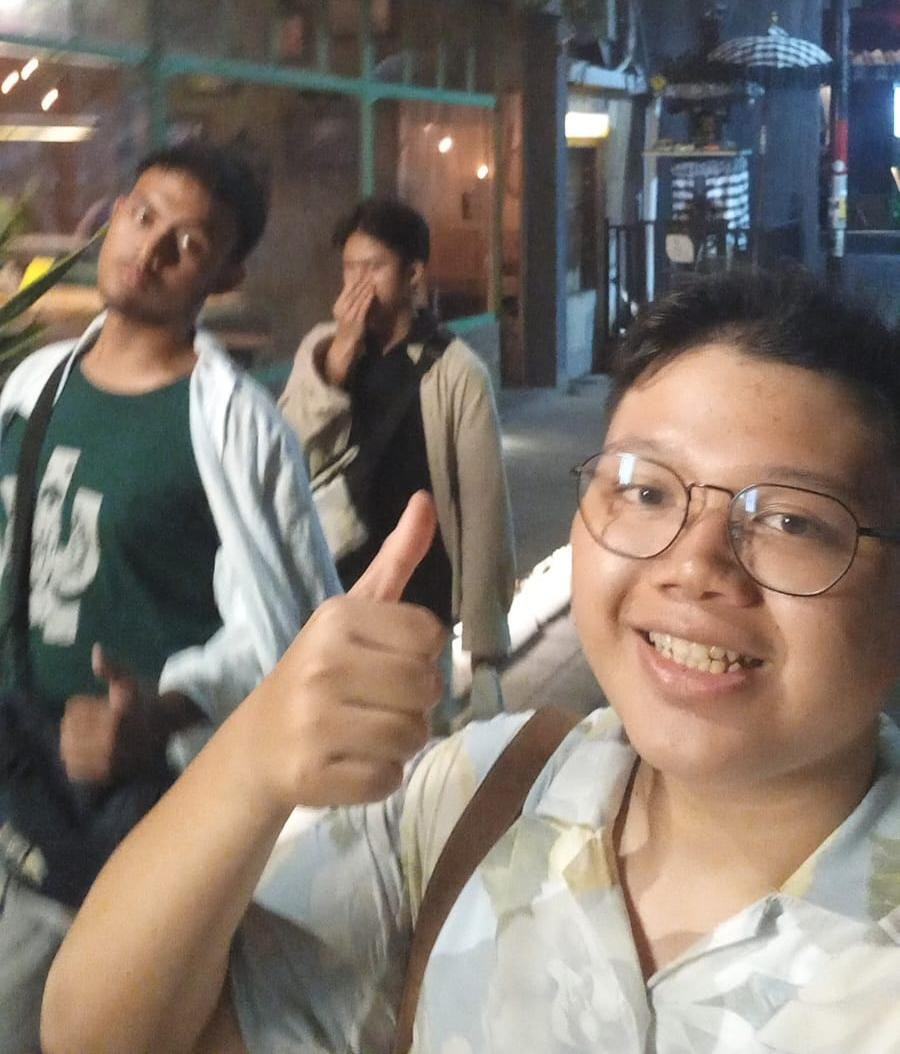
\includegraphics[width=0.6\linewidth,height=\textheight,keepaspectratio]{My_Stories_for_You/../images/myFriends.jpg}
\end{center}

Malam itu, setelah melewati berbagai kegiatan dalam rangkaian study tour
yang dinantikan para siswa, saya dan dua teman sekamar memutuskan untuk
berjalan kaki dari hotel menuju Pantai Kuta. Sebenarnya, saya ingin
menggunakan kendaraan dari aplikasi daring, tetapi kedua teman saya
bersikeras ingin berjalan kaki, meskipun waktu sudah cukup larut.
Setelah dibujuk dengan alasan bahwa momen seperti ini tidak akan
terulang lagi, saya akhirnya setuju. Ada sesuatu yang menarik dalam ide
berjalan menembus malam di tengah kota wisata yang ramai itu.

Perjalanan dimulai dengan langkah-langkah kecil di trotoar yang sepi dan
agak gelap. Satu-satunya cahaya berasal dari lampu kendaraan yang
sesekali melintas. Berdasarkan peta, kami diarahkan ke jalan sempit yang
hanya cukup untuk satu mobil. Namun, semakin jauh kami melangkah,
suasana kota mulai berubah dari sunyi menjadi hidup kembali. Suara musik
terdengar dari berbagai restoran, wisatawan asing tertawa, dan pedagang
di pinggir jalan menawarkan jasa pijat, terapi ikan, serta aneka cendera
mata. Keramaian itu membuat perjalanan terasa hangat. Kami terus
bercanda dan tertawa, menertawakan hal-hal kecil yang kami temui di
sepanjang jalan.

Meski begitu, ada juga saat-saat ketika suasana tiba-tiba berubah
hening. Jalanan yang sebelumnya ramai menjadi sepi. Kami hanya ditemani
langkah kaki sendiri dan hembusan angin malam. Ada sedikit rasa canggung
dan takut, tetapi anehnya terasa menenangkan. Mungkin karena untuk
pertama kalinya, saya benar-benar menikmati kebersamaan dalam
keheningan.

Setelah sekitar tiga puluh menit berjalan, kami akhirnya tiba di Pantai
Kuta. Rasa lelah seketika hilang, berganti dengan tawa lega dan
kebahagiaan yang sulit dijelaskan. Kami duduk di atas pasir, berbagi
cerita, dan menikmati suara ombak di tengah gelapnya malam. Tak lama
kemudian, rombongan lain datang dan terkejut mengetahui bahwa kami
menempuh perjalanan sejauh itu hanya dengan berjalan kaki. Kami tertawa
bersama, seolah perjalanan itu sendiri sudah menjadi bagian dari cerita
yang akan selalu diingat.

Tidak lama kemudian, lampu sorot di pantai mulai dimatikan sebagai tanda
bahwa waktu sudah terlalu malam. Kami pun memutuskan untuk kembali ke
hotel, kali ini dengan hati yang hangat dan pikiran yang penuh kenangan.

Malam itu mengajarkan saya sesuatu yang sederhana namun bermakna: kadang
keberanian tidak selalu datang dari menghadapi hal besar, melainkan dari
keputusan kecil untuk melangkah bersama. Saya yang awalnya ragu dan
takut akhirnya menyadari bahwa justru keputusan spontan itulah yang
menghadirkan kenangan paling berharga. Perjalanan ke Pantai Kuta bukan
sekadar perjalanan fisik, tetapi juga perjalanan batin menuju keberanian
dan kebersamaan yang tulus.

\begin{center}\rule{0.5\linewidth}{0.5pt}\end{center}

\section{Refleksi Diri}\label{refleksi-diri-1}

Dari pengalaman itu, saya belajar bahwa kadang keputusan kecil yang
impulsif justru membawa makna besar dalam hidup.\\
Saya yang awalnya pesimis dan takut berjalan di malam hari ternyata bisa
menikmati setiap langkah, bahkan bersyukur telah melakukannya.

Perjalanan ini juga membuat saya sadar bahwa rasa nyaman tidak selalu
berarti aman, dan terkadang kita perlu keluar dari kebiasaan untuk
menemukan sesuatu yang baru.\\
Lebih dari sekadar ke pantai, malam itu adalah perjalanan menuju
keberanian dan kebersamaan.

\begin{center}\rule{0.5\linewidth}{0.5pt}\end{center}

\section{Sentuhan Personal}\label{sentuhan-personal}

Saya masih ingat ketika kami bercanda di tengah jalan gelap, meniru gaya
turis yang sedang bernyanyi di restoran pinggir jalan. Salah satu teman
saya bahkan berkata,

\begin{quote}
``Kalau kita nyasar, yasudah sih\ldots{} Gak tau''
\end{quote}

Ucapan itu membuat kami tertawa keras-keras, dan sejak saat itu, setiap
kali melihat jalan malam yang sunyi, saya selalu teringat malam itu di
Kuta.

\begin{center}\rule{0.5\linewidth}{0.5pt}\end{center}

\section{Pesan untuk Pembaca}\label{pesan-untuk-pembaca}

Dari kisah sederhana ini, saya ingin menyampaikan bahwa setiap langkah
kecil yang kita ambil bersama orang lain dapat menjadi kenangan besar di
masa depan.\\
Tidak semua keberanian datang dari hal besar. Kadang, ia muncul dari
keputusan spontan untuk menikmati hidup apa adanya, bahkan jika itu
hanya sekadar berjalan kaki menuju pantai di malam hari.

\bookmarksetup{startatroot}

\chapter{UTS-4 My SHAPE (Strengths, Heart, Abilities, Personality,
Experiences)}\label{uts-4-my-shape-strengths-heart-abilities-personality-experiences}

\section{Identitas Diri}\label{identitas-diri-1}

\begin{itemize}
\tightlist
\item
  \textbf{Nama:} Muhammad Azikra Wira Pratama\\
\item
  \textbf{NIM:} 18224089
\item
  \textbf{Kelas:} K-01
\end{itemize}

\begin{center}\rule{0.5\linewidth}{0.5pt}\end{center}

\section{Hasil Tes VIA Character
Strengths}\label{hasil-tes-via-character-strengths}

Tautan : \href{StrengthsProfile-MuhammadAzikra-WiraPratama.pdf}{HASIL
TES}

\begin{center}\rule{0.5\linewidth}{0.5pt}\end{center}

\section{Pernyataan Misi Pribadi}\label{pernyataan-misi-pribadi}

\begin{quote}
``Saya ingin menjadi seseorang yang menggunakan kemampuan teknologi
untuk menciptakan solusi yang berdampak positif bagi masyarakat. Positif
ini tidak hanya mencakup dampak positif secara kehidupan namun
perkembangan masyarkat mulai dari cara berpikir untuk mau berkembang dan
memiliki rasa manusiawi.''
\end{quote}

\begin{center}\rule{0.5\linewidth}{0.5pt}\end{center}

\section*{Strengths (S)}\label{strengths-s}
\addcontentsline{toc}{section}{Strengths (S)}

\markright{Strengths (S)}

Saya memiliki kekuatan utama dalam apresiasi terhadap keindahan dan
keunggulan, pertimbangan, kerja sama tim, spiritualitas, rasa syukur,
keadilan, harapan, keingintahuan, dan kerendahan hati.

Saya menghargai keindahan dalam karya, alam, dan kehidupan sehari-hari,
serta berusaha untuk melakukan segala hal dengan sepenuh hati.

Saya cenderung berpikir matang sebelum bertindak, selalu menimbang sudut
pandang berbeda agar keputusan saya objektif.

Dalam kerja tim, saya menjaga komitmen, mendukung anggota lain, dan
berkontribusi untuk mencapai tujuan bersama.

Nilai spiritual memberi arah bagi saya, membuat saya tetap tenang dalam
menghadapi tantangan.

Saya juga mudah bersyukur, menghargai hal kecil, dan menjunjung keadilan
dalam memperlakukan orang lain.

Harapan dan rasa ingin tahu membuat saya selalu optimis dan tertarik
untuk belajar hal baru, sementara kerendahan hati membantu saya menerima
masukan dengan terbuka.

\begin{center}\rule{0.5\linewidth}{0.5pt}\end{center}

\section*{Heart (H)}\label{heart-h}
\addcontentsline{toc}{section}{Heart (H)}

\markright{Heart (H)}

Saya memiliki gairah yang besar terhadap kreativitas, refleksi, dan
kontribusi sosial.

Saya menikmati proses menciptakan sesuatu yang bermakna dan mencari cara
agar karya saya membawa manfaat bagi orang lain.

Nilai inti saya terletak pada kejujuran, empati, dan keinginan untuk
terus berkembang.

Saya merasa puas ketika dapat membantu orang lain menemukan potensi
mereka dan melihat dampak nyata dari kolaborasi yang baik.

\begin{center}\rule{0.5\linewidth}{0.5pt}\end{center}

\section*{Abilities (A)}\label{abilities-a}
\addcontentsline{toc}{section}{Abilities (A)}

\markright{Abilities (A)}

Saya memiliki kemampuan teknis di bidang pemrograman menggunakan Python,
C, dan Java.

Selain itu, saya terbiasa menggunakan logika dan pendekatan sistematis
dalam menyelesaikan masalah.

Dalam aspek non-teknis, saya mengandalkan kemampuan komunikasi yang
efektif dan kerja tim untuk menjaga alur kerja tetap efisien.

Saya percaya bahwa kemampuan bukan hanya tentang apa yang bisa
dilakukan, tetapi bagaimana kemampuan itu digunakan untuk memberikan
hasil yang bermanfaat bagi lingkungan sekitar.

\begin{center}\rule{0.5\linewidth}{0.5pt}\end{center}

\section*{Personality (P)}\label{personality-p}
\addcontentsline{toc}{section}{Personality (P)}

\markright{Personality (P)}

Saya termasuk tipe kepribadian \textbf{INFP} : reflektif, empatik, dan
idealis.

Saya lebih suka bekerja dengan makna yang jelas dan lingkungan yang
memberi ruang untuk berpikir dan berinovasi.

Saya senang berkolaborasi dengan orang lain, terutama ketika visi yang
dibangun bersama terasa bermakna dan positif.

Saya berorientasi pada nilai dan lebih menghargai proses dibanding
sekadar hasil akhir.

\begin{center}\rule{0.5\linewidth}{0.5pt}\end{center}

\section*{Experiences (E)}\label{experiences-e}
\addcontentsline{toc}{section}{Experiences (E)}

\markright{Experiences (E)}

Dari pengalaman berorganisasi, saya belajar pentingnya komunikasi yang
jujur dan koordinasi yang baik antaranggota tim.

Saya menyadari bahwa keberhasilan tidak hanya datang dari kemampuan
individu, tetapi juga dari rasa saling percaya dan tanggung jawab
bersama.

Dari dunia perkuliahan, saya belajar bahwa ilmu sangat luas dan menuntut
pola pikir terbuka.

Proses belajar bukan hanya tentang memahami teori, tetapi juga tentang
bagaimana menerapkannya dengan etika dan kesadaran diri.

\begin{center}\rule{0.5\linewidth}{0.5pt}\end{center}

\section{Refleksi Akhir}\label{refleksi-akhir}

\begin{quote}
\emph{Diriku yang esok hari ini harus menjadi lebih baik dari diriku
yang saat ini. Saya menggunakan pola pikir itu dalam menghadapi berbagai
hal dalam kehidupan.}
\end{quote}

\begin{center}\rule{0.5\linewidth}{0.5pt}\end{center}

\section{Catatan}\label{catatan}

Template ini menggunakan konsep \textbf{S-H-A-P-E}:

\begin{longtable}[]{@{}lll@{}}
\toprule\noalign{}
Huruf & Arti & Fokus \\
\midrule\noalign{}
\endhead
\bottomrule\noalign{}
\endlastfoot
\textbf{S} & Strengths & Kekuatan khas dan keunikan pribadi \\
\textbf{H} & Heart & Nilai inti dan hal yang kamu cintai \\
\textbf{A} & Abilities & Keterampilan utama (hard \& soft skills) \\
\textbf{P} & Personality & Profil kepribadian dan gaya kerja \\
\textbf{E} & Experiences & Pelajaran hidup dari pengalaman nyata \\
\end{longtable}

\bookmarksetup{startatroot}

\chapter{UTS-5 My Personal Reviews}\label{uts-5-my-personal-reviews}

Berikut cara saya melakukan review: mengguan chatGPT, saya mengattach
\href{skor_uts.pdf}{file promt ChatGPT}, disertai perintah : ``self
assess uts-1 sanpai uts-5 dari URL
`https://awp-confirm.github.io/all-about-me/'\,''

ChatGPT melakukan self-assessment UTS-1 s.d. UTS-5 langsung dari laman
yang Anda berikan dan menilai memakai rubrik tugas UTS (skala 1--5 per
kriteria). Rekap skor siap diunduh sebagai CSV:
\href{Self-Assessment_UTS-1_s_d__UTS-5__dibuat_otomatis_.csv}{Download
CSV ringkasan}.

\section{Hasil Self-Assessment UTS (URL:
https://awp-confirm.github.io/all-about-me/)}\label{hasil-self-assessment-uts-url-httpsawp-confirm.github.ioall-about-me}

\subsection*{Identifikasi}\label{identifikasi}
\addcontentsline{toc}{subsection}{Identifikasi}

\textbf{Nama Mahasiswa:} Muhammad Azikra Wira Pratama\\
\textbf{NIM:} 18224089\\
\textbf{Jenis Penilaian:} Self-assessment

\begin{center}\rule{0.5\linewidth}{0.5pt}\end{center}

\subsection*{Tinjauan Umum}\label{tinjauan-umum}
\addcontentsline{toc}{subsection}{Tinjauan Umum}

Seluruh bagian portofolio UTS telah tersusun lengkap dari UTS-1 hingga
UTS-5.\\
Setiap bagian menunjukkan perkembangan kemampuan komunikasi personal,
refleksi diri, dan penerapan konsep interpersonal.

Struktur portofolio mencakup: - \textbf{UTS-1 (All About Me):}
Menampilkan narasi reflektif dari identitas diri hingga penutup.\\
- \textbf{UTS-2 (My Songs for You):} Lagu pilihan \emph{``7 Years''}
disertai alasan, pesan personal, dan refleksi makna.\\
- \textbf{UTS-3 (My Stories for You):} Cerita pendek ``A Way to the
Beach'' dengan pendahuluan, inti, dan penutup reflektif.\\
- \textbf{UTS-4 (My SHAPE):} Menyajikan hasil tes VIA, misi pribadi,
serta refleksi S-H-A-P-E secara rinci.\\
- \textbf{UTS-5 (My Personal Reviews):} Analisis pesan dan evaluasi diri
menggunakan pendekatan komunikasi interpersonal.

\begin{center}\rule{0.5\linewidth}{0.5pt}\end{center}

\section*{Tinjauan Spesifik Per
Bagian}\label{tinjauan-spesifik-per-bagian}
\addcontentsline{toc}{section}{Tinjauan Spesifik Per Bagian}

\markright{Tinjauan Spesifik Per Bagian}

\subsection*{UTS-1 --- All About Me (95
\%)}\label{uts-1-all-about-me-95}
\addcontentsline{toc}{subsection}{UTS-1 --- All About Me (95 \%)}

\textbf{Kriteria Nilai:}\\
Orisinalitas = 5 Keterlibatan = 5 Humor = 4 Wawasan = 5

\textbf{Catatan \& Refleksi:}\\
Tulisan orisinal dan reflektif, dengan gaya personal kuat.\\
Perlu ditambah contoh konkret pada bagian \emph{Sisi Ringan} agar narasi
lebih hidup.

\begin{center}\rule{0.5\linewidth}{0.5pt}\end{center}

\subsection*{UTS-2 --- My Songs for You (90
\%)}\label{uts-2-my-songs-for-you-90}
\addcontentsline{toc}{subsection}{UTS-2 --- My Songs for You (90 \%)}

\textbf{Kriteria Nilai:}\\
Orisinalitas = 4 Keterlibatan = 5 Humor = 4 Inspirasi = 5

\textbf{Catatan \& Refleksi:}\\
Pilihan lagu \emph{``7 Years''} relevan dengan tema refleksi diri.\\
Akan lebih bermakna bila ditambah momen pribadi saat lagu ini terasa
signifikan.

\begin{center}\rule{0.5\linewidth}{0.5pt}\end{center}

\subsection*{UTS-3 --- My Stories for You (95
\%)}\label{uts-3-my-stories-for-you-95}
\addcontentsline{toc}{subsection}{UTS-3 --- My Stories for You (95 \%)}

\textbf{Kriteria Nilai:}\\
Orisinalitas = 5 Keterlibatan = 5 Pengembangan Narasi = 4 Inspirasi = 5

\textbf{Catatan \& Refleksi:}\\
Kisah menggambarkan perjalanan dan pertumbuhan diri dengan baik.\\
Disarankan menambahkan satu konflik kecil agar ketegangan emosional
meningkat.

\begin{center}\rule{0.5\linewidth}{0.5pt}\end{center}

\subsection*{UTS-4 --- My SHAPE (85 \%)}\label{uts-4-my-shape-85}
\addcontentsline{toc}{subsection}{UTS-4 --- My SHAPE (85 \%)}

\textbf{Kriteria Nilai:}\\
Orisinalitas = 4 Keterlibatan = 4 Pengembangan Narasi = 4 Inspirasi = 5

\textbf{Catatan \& Refleksi:}\\
Setiap komponen S-H-A-P-E telah dijelaskan dengan sistematis.\\
Akan lebih kuat jika ditambah pengalaman nyata yang mencerminkan
kekuatan diri.

\begin{center}\rule{0.5\linewidth}{0.5pt}\end{center}

\subsection*{UTS-5 --- My Personal Reviews (80
\%)}\label{uts-5-my-personal-reviews-80}
\addcontentsline{toc}{subsection}{UTS-5 --- My Personal Reviews (80 \%)}

\textbf{Kriteria Nilai:}\\
Pemahaman Konsep Interpersonal = 4 Analisis Kritis Pesan = 4 Argumentasi
(Logos) = 4 Etos \& Empati = 4 Rekomendasi Perbaikan = 4

\textbf{Catatan \& Refleksi:}\\
Analisis menunjukkan pemahaman konsep interpersonal yang baik.\\
Gunakan pola tetap: \emph{tujuan -- audiens -- hal efektif -- aspek
perbaikan -- langkah konkret.}

\begin{center}\rule{0.5\linewidth}{0.5pt}\end{center}

\section*{Skor dan Ringkasan
Penilaian}\label{skor-dan-ringkasan-penilaian}
\addcontentsline{toc}{section}{Skor dan Ringkasan Penilaian}

\markright{Skor dan Ringkasan Penilaian}

\begin{longtable}[]{@{}llllll@{}}
\toprule\noalign{}
UTS & Skor & CPMK-1 & CPMK-2 & CPMK-3 & CPMK-4 \\
\midrule\noalign{}
\endhead
\bottomrule\noalign{}
\endlastfoot
UTS-1 & 95 & 3.80 & 5.70 & 0.00 & 0.00 \\
UTS-2 & 90 & 4.50 & 6.30 & 0.00 & 0.00 \\
UTS-3 & 95 & 5.70 & 6.65 & 0.00 & 0.00 \\
UTS-4 & 85 & 5.95 & 5.10 & 0.00 & 0.00 \\
UTS-5 & 80 & 6.40 & 8.00 & 0.00 & 0.00 \\
\end{longtable}

\textbf{Total Kontribusi CPMK:}\\
CPMK-1 = 26.35  CPMK-2 = 31.75  CPMK-3 = 0.00  CPMK-4 = 0.00

\begin{center}\rule{0.5\linewidth}{0.5pt}\end{center}

\section*{Refleksi Akhir}\label{refleksi-akhir-1}
\addcontentsline{toc}{section}{Refleksi Akhir}

\markright{Refleksi Akhir}

Melalui seluruh proses UTS ini, saya belajar bahwa refleksi diri bukan
hanya sekadar menulis tentang pengalaman, tetapi juga memahami
nilai-nilai yang membentuk cara berpikir dan berinteraksi.\\
Setiap bagian portofolio menunjukkan sisi berbeda dari diri saya ---
mulai dari mengenal jati diri, memaknai lagu, hingga menilai kekuatan
pribadi dan cara berkomunikasi.

Proses ini menegaskan bahwa komunikasi efektif tidak hanya tentang
berbicara, tetapi juga tentang memahami, berempati, dan belajar dari
setiap interaksi.\\
Saya berkomitmen untuk terus mengembangkan kemampuan ini di masa depan
agar dapat menjadi pribadi yang lebih reflektif, terbuka, dan bermanfaat
bagi lingkungan sekitar.

\bookmarksetup{startatroot}

\chapter{UAS-1 My Concepts}\label{uas-1-my-concepts}

Mau hidup epik ? \href{lifestory.pdf}{Write your Life Story}

Apa itu berkonsep?

\url{https://youtu.be/QVfUlVBO80U?si=yM6q_rwV9rcDBbu7}

\bookmarksetup{startatroot}

\chapter{UAS-2 My Opinions}\label{uas-2-my-opinions}

SApa itu beropini? \href{BM\%20Opini.mp4}{Opini Berpengaruh}

Bagiamana menjaadi menarik? \href{./Interesting.mp4}{Menjadi Menarik}

\bookmarksetup{startatroot}

\chapter{UAS-3 My Innovations}\label{uas-3-my-innovations}

\bookmarksetup{startatroot}

\chapter{UAS-4 My Knowledge}\label{uas-4-my-knowledge}

Cara saya mengkomunikasikan sebuah pengatahuan sebagai petunjuk bagi
orang lain 1) saya tulis
\href{Rekomendasi\%20Presentasi\%20Efektif(Contoh\%20Makalah).pdf}{makalah
sebagai bahan utama} 2) lalu saya buat
\href{Contoh\%20Transkrip\%20Presentasi.pdf}{transkrip ucapan lisan} 3)
kemudian saya kembangkan
\href{Rekomendasi\%20Presentasi\%20(Contoh\%20Slides).pdf}{slide
pendukung trnsskrip} 4) lalu saya memproduksivideo audio visual
\url{https://youtu.be/ZbghfMvnPZc} \url{https://youtu.be/ZbghfMvnPZc}

\bookmarksetup{startatroot}

\chapter{UAS-5 My Professional
Reviews}\label{uas-5-my-professional-reviews}

Untuk melkukan review, seperti pada
\href{../My_Personal_Reviews/Doc.5.Mengevaluasi-Esai-Berdasarkan-Rubrik.pdf}{pendekatan
AI}, kita membutuhkan rubrik - Rubrik
\href{Dok.4.a.Rubrik_Kisah.pdf}{Kisah} - Rubrik
\href{Dok.4.b.Rubrik_Konsep.pdf}{Konsep} - Rubrik
\href{Dok.4.c.Rubrik_Opini.pdf}{Opini}

\bookmarksetup{startatroot}

\chapter{Summary}\label{summary}

In summary, this book has no content whatsoever.

\bookmarksetup{startatroot}

\chapter*{References}\label{references}
\addcontentsline{toc}{chapter}{References}

\markboth{References}{References}

\phantomsection\label{refs}




\end{document}
